\documentclass[sigplan, screen]{acmart}
\AtBeginDocument{%
  \providecommand\BibTeX{{%
    \normalfont B\kern-0.5em{\scshape i\kern-0.25em b}\kern-0.8em\TeX}}}



\usepackage{subfigure}
\usepackage{caption}

%%
%% end of the preamble, start of the body of the document source.
\begin{document}

%%
%% The "title" command has an optional parameter,
%% allowing the author to define a "short title" to be used in page headers.
\title{Generating Trigger-Action Program from Traces\\Based on Association Rule Mining: A Survey}

%%
%% The "author" command and its associated commands are used to define
%% the authors and their affiliations.
%% Of note is the shared affiliation of the first two authors, and the
%% "authornote" and "authornotemark" commands
%% used to denote shared contribution to the research.
\author{Yicheng Wang}
\affiliation{%
  \institution{Institute of Software \\ Chinese Academy of Sciences}
  \city{Haidian Qu}
  \state{Beijing}
  \country{China}
}
\email{wangyicheng215@mails.ucas.ac.cn}

%%
%% By default, the full list of authors will be used in the page
%% headers. Often, this list is too long, and will overlap
%% other information printed in the page headers. This command allows
%% the author to define a more concise list
%% of authors' names for this purpose.
\renewcommand{\shortauthors}{Yicheng Wang}

%%
%% The abstract is a short summary of the work to be presented in the
%% article.
\begin{abstract}
  Trigger-action programming (TAP) is a novel approch to define connections between different Internet of Things (IoT) devices and services,
  which could translate human’s intent of IoT devices into desired automation. User-written TAP rules have been widely used
  as a programming interface in popular IoT systems.
  As users may experience difficulties in discovering related devices functionality and designing rules, recent works try to
  automatically generate TAP rules from past user event traces (time-stamped logs of sensor readings and manual actuations of devices).
  which turns problem into association rule mining of user's trace sequences.

  This survey presents a taxonomy of classic association rule mining (ARM) algorithms, indicates the basic workflow and the important key features of these
  representative algorithms. We also investigate the meritorious applications in Ambient Intelligence (AmI) area, which utilize ARM algorithms to mining the frequent 
  pattern in user event traces, and classify the applications by the algorithms they use. This survey serves as an introduction for IoT related researchers who 
  are intend to realize smart device automation by past behavior mining, and we identifies notable opportunities for further work.


  
\end{abstract}

%%
%% The code below is generated by the tool at http://dl.acm.org/ccs.cfm.
%% Please copy and paste the code instead of the example below.
%%
\begin{CCSXML}
<ccs2012>
 <concept>
  <concept_id>10010520.10010553.10010562</concept_id>
  <concept_desc>Computer systems organization~Embedded systems</concept_desc>
  <concept_significance>500</concept_significance>
 </concept>
 <concept>
  <concept_id>10010520.10010575.10010755</concept_id>
  <concept_desc>Computer systems organization~Redundancy</concept_desc>
  <concept_significance>300</concept_significance>
 </concept>
 <concept>
  <concept_id>10010520.10010553.10010554</concept_id>
  <concept_desc>Computer systems organization~Robotics</concept_desc>
  <concept_significance>100</concept_significance>
 </concept>
 <concept>
  <concept_id>10003033.10003083.10003095</concept_id>
  <concept_desc>Networks~Network reliability</concept_desc>
  <concept_significance>100</concept_significance>
 </concept>
</ccs2012>
\end{CCSXML}

\ccsdesc[500]{Human-centered computing~Ambient intelligence}
\ccsdesc[500]{Human-centered computing~Ubiquitous and mobile computing}
\ccsdesc[500]{Software and its engineering~General programming languages}
\ccsdesc[500]{Information systems~Data mining}
\ccsdesc[500]{Information Storage and Retrieval~Retrieval models}

%%
%% Keywords. The author(s) should pick words that accurately describe
%% the work being presented. Separate the keywords with commas.
\keywords{Trigger-action programming, Internet of Things, Event prediction, Association Mining, Sequential Pattern Mining}

%%
%% This command processes the author and affiliation and title
%% information and builds the first part of the formatted document.
\maketitle
\section{Introduction}
The goal of Ambient Intelligence (AmI) is to realize smart interactive environments which could assist us in our everyday 
tasks, as reacting to our commands and predicting our behavior. The achievement of this goal is advancing with the developement
of artificial intelligence techniques and the popularization of Internet of Things (IoT). Plenty of machine learning algorithms
have been used in \textbf{behaviour modelling and prediction}, including probabilistic graphical models\cite{mohmed2020enhanced, nazerfard2012bayesian, wu2016behavior},
imitation learning\cite{minor2015data, minor2017learning},neural network\cite{tax2018human, xu2016user}. This survey mainly focus 
on rule-based AmI implementation\cite{pentland1999modeling, jakkula2007mining}, which determining what tasks are likely to be done next and doing them
according to context-dependent rulesets, translate user’s intent of IoT devices into desired automation.


\textbf{Trigger-action programming (TAP)}\cite{ghiani2017personalization, huang2015supporting, ur2014practical} is a novel rule-based approch 
that provide interfaces for users to create personalized rulesets. TAP is in form of if-this-then-that (e.g., “IF trigger occurs WHILE conditions are true, THEN take
 some action”), which is available on most popular IoT systems including IFTTT\cite{IFTTT}, Microsoft Flow\cite{levy2017microsoft},
  Samsung SmartThings\cite{mossberg2014smartthings}, etc. These interface offer non-technical users the opportunity to define the connection between different IoT 
  devices and to automate smart spaces in simple scenarios. 

However, there are limitations having users write rules. Firstly, users writing rules may contain bugs or otherwise fail to match their intent\cite{mikolov2016roadmap, antonakakis2017understanding}.
Furthermore, users often find it hard to reason about how sensors (e.g., motion sensors) in smart homes work. Tools have been developed to assist users writing TAP rules and 
detecting bugs in TAP programs\cite{luo2020arbee, lien2016soli}, while it is difficult in the general case to solve the problems above. Therefore,
recent works try to generate TAP rules or predict user activities based on traces automatically.

Normally, traces of IoT devices are time-stamped logs of sensor readings and manual actuations of devices. The basic idea of smart space automation 
is taking traces as input, mining the frequent and valuable patterns in the trace, recording these patterns as event-driven rules, regarding the proper features
in the pattern as \emph{Trigger, Condition} and \emph{Action} of rules. 


\begin{itemize}
  \item \textbf{Memory segement}: \emph{byte} type array of fixed size 32K;
  \item \textbf{Memory block}: \emph{long} type array of required data size;
  \item \textbf{Cached RDD}: Array of user-defined type with required length, each element is of user-defined type.
\end{itemize}

Modern big data processing frameworks, including Hadoop\cite{shvachko2010hadoop}, Spark\cite{zaharia2010spark} and
Flink\cite{carbone2015apache}, were all implemented in object-oriented languages such as Scala and Java, due to 
theirs applicability across heterogeneous distributed clusters, convenience on memory management, and fertility 
of community resources. However, big data applications suffer from striking high GC cost under JVM. As reported by users and researchers,
GC time can take even more than 50$\%$ of the overall application execution time in some cases\cite{stackoverflow, bu2013bloat}.
Some concurrent GC algorithms, e.g., G1 GC\cite{detlefs2004garbage}, are able to limit GC pause times to a certain extent, 
while mutator threads would be inevitably affected\cite{xu2019experimental, wu2020platinum}.

The GC inefficiency problem under big data processing frameworks has been widely studied\cite{xu2019experimental,bruno2018study,gidra2013study}, 
and results from a combination of factors. First, big data applications are both \emph{data-intensive} and \emph{memory-intensive}, a large amount of data 
is loaded in the memory as objects at the runtime, putting servere overhead on the GC colloctor. Big data processing frameworks that caching intermediate 
computing results in the memory make thins even worse.
 Second, the memory usage pattern of big data applications is totally different from traditional Java applications, data objects of big data applications tend to stay in memory
 for a long period of time, which is opposite to the\emph{weak generational hypothesis hypothesis}\cite{weakgenerational} that the classical GC algorithms based on.
 
The weak generational hypothesis states that most objects survive for a short time and only a few objects live long. For this reason, popular GC colloctors
are implemented generational, i.e., divide the heap into generations, typically young generation for keeping short-lived objects, and old
generation for keeping long-lived objects. Thus by collecting the young generation more frequently than old generation, GC colloctors reduce the average number of objects 
processed per GC cycle. 

Under generational GC algorithms, long-lived data obejcts are destined to survive in \emph{minor GC} cycles, which is target at young generation,
and certain to be promoted to the old generation eventually when their survival times reach a certain threshold. In each GC cycle, all the long-lived data obejcts would be marked
as "live" objects by the \emph{accessibility analysis} across the object reference graph, and be compacted (copied) to another memory space. Even after being promoted, these
long-lived obejcts would still not be "dead" in a short time, while their big volume makes it very likely to trigger \emph{major GC} when the old generation is full, 
which introduces more unnecessary scan and copy of them. 
As objects marking and moving are considered to be the most time-consuming part of the GC cycle\cite{suo2018characterizing,yu2016performance}, the long-lived data objects is regarded
as the main reason to the degradation of GC efficiency and the main direction of optimization.

Moving back to unmanaged languages and leave memory management to developers is a tiring but possible solution\cite{chenSM,maas2017return}. However, unmanaged languages are error-prone,
espicially to big data applications whose memory usgae is stressful and complicated and whose running time is quite long. Furthermore, since a great number of existing
big data processing frameworks are already developed in a managed language, it is unrealistic to re-implement once again\cite{nguyen2015facade,bruno2018study}. Some other works
 attempt to use the APIs from package \emph{sun.misc.Unsafe} to handle the off-heap memory explicitly like unmanaged languages\cite{mastrangelo2015use,navasca2019gerenuk,nguyen2015facade}.
 The problem is that, as the warning of its name, \emph{Unsafe} package is unsafe. It has the drawbacks same as unmanaged languages, and it may introduce serialization/deserialization
 jobs in orginal big data environment. Therefore, more works still settle the long-lived objects in heap.Two main optimization techniques used in these work are lifetime-based 
 memory management and region-based memory management. The former obtains the lifetime of data objects by static analysis of source code and users' annotation, reclaim the 
 long-lived objects at their "dead" point in the code. The latter leverages the lifetime information to divide the data obejcts by their live time into separate memory spaces, 
 facilitates one-time reclamation\cite{lu2016lifetime,kolokasis2020say,nguyen2016yak,cohen2015data,wang2019panthera}. 
 
Inspired by the techniques above, we pick out the long-lived objects according to the lifetime information, and pretenure them in the older generation. As G1 GC are naturely region-based,
we directly create a new generation aiming at the storage of long-lived data objects on the top of G1, whose regions would neither be involved in minor GC, nor be in the collection sets of major GC, unless it get the signal that the lifetime of the objects in current region is end. 
Thanks to Spark Tungsten\cite{Tungsten} project and Flink who utlizing primitive arraies as memory
pages to form unmanaged-languages-like condition on heap, we could readily pretune most long-lived data by pretuning memory page objects(primitive arraies). We evalute our idea 
by the time costed to creat memory pages. Result shows that, compared with orginal G1 GC, we eliminated 90$\%$ of minor GC pause time.

\section{Motivation}
The main challenge of pretenuring in JVM is determining the long-lived objects. Previous pretenuring works using sampling\cite{harris2000dynamic,jump2004dynamic}, profiling\cite{blackburn2001pretenuring,bruno2019runtime,bruno2017polm2} 
and annotation\cite{bruno2017ng2c} to speculate the lifetime of all the objects. These approches inevitably introduce repeat executions, CPU competition or heavy users' efforts, many of works are highly dependent on the users' developement experience
and knowledge on GC algorithm. Fortunately, long-lived objects determination is simpler under big data processing framworks for the characteristics below:

\subsection{Data Path}

More than 95$\%$ of runtime objects are created and used by a rather small and simple code referred as \emph{data path}, that primarily conducts data manipulation like map, 
reduce, and relational operations. The objects created by \emph{data path} are \emph{data objects}, which are the main component of a long-lived objects. Only less than 5$\%$
 of runtime objects are created by a large and complex code referred as \emph{control path}.The \emph{control objects} created by \emph{control path} are principally 
 for cluster management, scheduling, communication, and others, which are basiclly short-lived and negligible\cite{nguyen2015facade,navasca2019gerenuk,bu2013bloat,nguyen2016yak}. This insight
 allow us focus on a small amount of code when handling long-lived data objects in big data applications, rather than pay attention to massive code in ordinary Java applications.

\subsection{Memory Pages}

As storing the data as objects requires additional memory footprint, some works use primitive array as memory pages to store the data value only. 
The structure of a data object in the JVM contains object headers and references to other objects, and the data value itself usually takes up no more than half of the space 
in the object\cite{navasca2019gerenuk,bu2013bloat}. For the reason that the methods of the data object are seldom used, the "shells" of objects is not only meaningless, but also harmful as it 
introduces serialization/deserialization work when the data is transformed across the cluster through the network, which may accounte for 30$\%$ of the total execution time\cite{navasca2019gerenuk,nguyen2018skyway}   
Therefore, these works allocate primitive array as memory page or memory container, gather the data with similar lifetime in the same memory page, and manage the long-lived data 
as a whole by managing the memory page objects\cite{navasca2019gerenuk,bu2013bloat,nguyen2015facade,lu2016lifetime}, reclaim the memory pages at the end of iterations, stages and
computing operators.

\begin{figure*}
  \centering
  \subfigure[Memory Block of Spark]{
    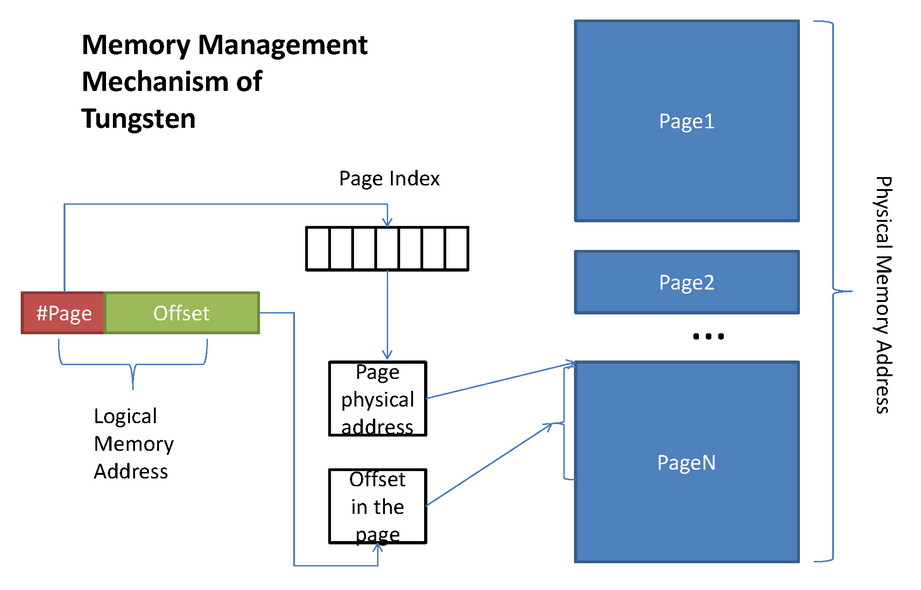
\includegraphics[width=0.45\textwidth]{figures/memoryblock}
  } 
  \subfigure[Memory Segment of Flink]{
    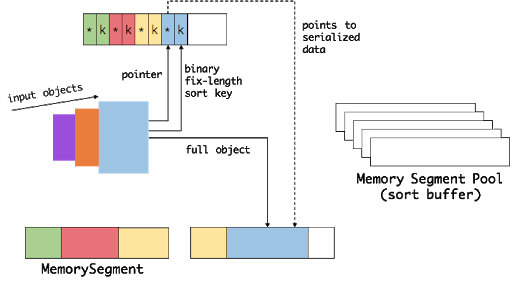
\includegraphics[width=0.45\textwidth]{figures/memorysegement}
  } 
  \caption{Memory Page in Modern Big Data Processing Framworks.}
\end{figure*}

Modern big data processing framworks utilized the idea of memory page, store the serialized data value in the memory page. As shown in Figure 1(a), Tungsten project of Spark uniform the in-heap and off-heap memory by memory blocks,
Tungsten manages memory blocks as page table. The memory location of a data value is determined by the page number and the offset in page. Off-heap page number is represented by an 
absolute address, and the page offset is the current address. On-heap page number is represented by the reference to the corresponding array object, and the offset in page 
is the relative offset within the array object. When the data in the page are freed explicitly by Spark, the memory page object would be added to a memory pool made up by weak reference, 
which means the memory page either be reused before it is scanned, or be relcaimed in next GC cycle. 

Similar to Spark Tungsten, Flink serializes objects into a fixed number of memory segments. As shown in Figure 1(b), memory manager of Flink holds a huge collection of 
memory segments in the memory pool. Different from memory blocks of Spark, memory segment is pre-allocated and fixed-sized, whose default size is 32KB. In addition, the lifetime of memory segments in the memory pool is 
same as computing task, it would only be released when the task end.

Design of memory page brings remarkable performance improvement to the big data processing frameworks, the reasons are as follows. (1) The binary form of data in memory page increases the storage density of memory, which allows more data cached
in the memory. The employment of memory page decreases the number of objects, i.e., reduces the pressure of GC. (2) The frameworks implements specialized serializer and computing
operators aiming at binary data speed up the execution and data transmission. (3) The continuous arrangement of data in memory page improves the spatial locality of memory accessment, 
 which is a great concern of current GC algorithm for it improves L1/L2/L3 cache hit ratio of CPU\cite{yang2020improving,li2019scissorgc}. 
 
 The contradiction is the choice between on-heap and off-heap, which are both available in Flink and Spark. The benefits of using off-heap are attractive, nevertheless the usage of off-heap is not safe and secure under big data frameworks as discussed in section 1, and Java Unsafe package is not available since JDK 11\cite{UnsafeRemove}. 
 Therefore, allocating memory pages on heap is the most likely direction for the future. The left problem is, the cost of promoting memory pages and major GC is still noteworthy
 in a large memory environment\cite{MinorGCLong}, which can be solved exactly by pretenuring. The clear type and size of memory page makes this work achievable.

\section{Desgin and Implementation}
  We implement our idea in the OpenJDK 8 HotSpot JVM, one of the most widely used industrial JVMs. Since HotSpot is a highly optimized production JVM, our algorithms were implemented carefully
to prevent the other function and the overall performance of JVM, some analysis and choices are made during the implementation procedure. Essential details are as follows.

\subsection{Pick Out Long-Lived Objects}
  Cached records and accumulated shuffled records are the main source of long-lived data objects in big data processing framworks\cite{xu2019experimental}. Cached records stand for
reusable data which are retained in memory by developers, in order to reduce disk I/O. Developer explicitly caching data using method \emph{cache()} or \emph{persist()}, and release them 
from memory using method \emph{unpersist()}. Cached \emph{Resilient Distributed Dataset} (RDD) in Spark is a typical example that we focus on. The lifetime of shuffled records
is more complicated, nevertheless, they are handled in memory pages. Therefore, we can only focus on memory block and memory segment.

As discussed in section 2.1, the manipulation of data objects is accomplished by a few code in data path. There is no exception on cached RDD, memory block and memory segement.
The building function of these three kinds of objects are respectively:  
\begin{itemize}
  \item \textbf{Memory segement}: \emph{byte} type array of fixed size 32K;
  \item \textbf{Memory block}: \emph{long} type array of required data size;
  \item \textbf{Cached RDD}: Array of user-defined type with required length, each element is of user-defined type.
\end{itemize}

The next job is letting JVM figure out thses long-lived objects at runtime. Dispose of memory segement and memory block is rather straightforward, as they are primitive types array, 
the creation of them are done by corresponding initialed \emph{TypeArrayKlass} in JVM, respectively \emph{byteArrayKlassObj} and \emph{longArrayKlassObj}. For the memory segement 
is fixed-sized, we identify it by the size when allocating. Though the length of memory block varies, it is generally longer than the length of ordinary long type array, we identify a long type array memory
block if its length exceeds a threshold, the rest memory blocks whose length smaller than threshold are rather negligible. Dispose of cached RDD is rather difficult, for the element object of cached RDD may contain 
variety types of objects, we only handle the RDD array. Even so, we still can not identify it without the help from code of big data processing frameworks. We pass the user-defined type \emph{T}
 to the JVM, and identify \emph{T} type array cached RDD if its length exceeds threshold, which is a common approch to identify RDD array\cite{wang2019panthera}.         

\subsection{GC Colloctor Choice}
After figured in the JVM, the allocation request of long-lived object is passed to the allocator, which varies from GC algorithm. There are two reasonable choice: 
Parallel scavenge GC and G1 GC, two most widely used GC collectors in HotSpot. Parallel is the default collector of JDK 8, which is the most popular version of JDK. 
G1 is the default collector since JDK 9, and is explicitly set as the default collector in Flink.

As shown in Figure 2, the distinct difference between Parallel and G1 is that, the young and old generations are both contiguous space with an explicit boundary in Parallel, and major GC would handle the whole heap space, while G1 logically separates young and old generations in a non-contiguous way, by dividing
heap space into a large number of equal-sized regions, each region can be young or old space, only some garbage-filled heap regions picked in the collection
 set would be handled during most major GC. Specially, Parallel store humongous objects directly into old generation, and G1 stores humongous objects 
 into humongous regions, which span multiple regions in old generation.
\begin{figure}[h]
  \centering
  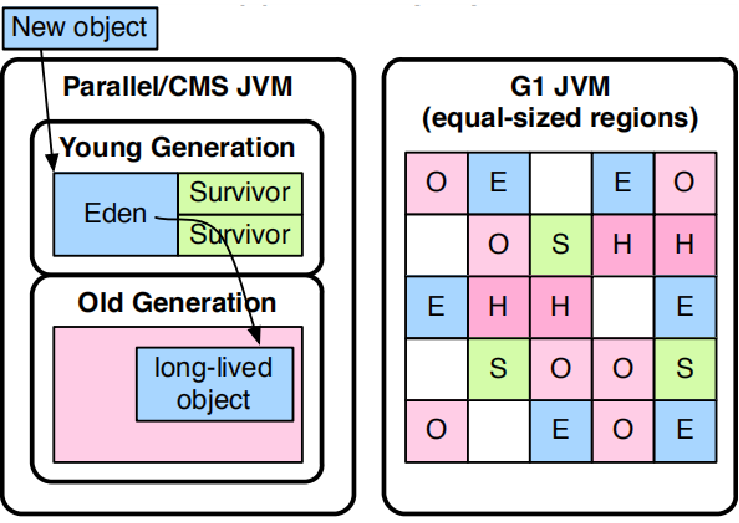
\includegraphics[width=\linewidth]{figures/GCalgorithm}
  \caption{Heap distribution under Parallel scavenge GC and G1 GC algorithm}
\end{figure}
Pretuning is easy to implement in Parallel GC, as the method of humongous objects allocation is relatively exposed, using this method could directly settle the
long-lived memory pages in the old generation without the modification of heap lock in JVM. However, memory pages pretuned in Parallel are mixed with other
ordinary objects promoted in old generation, still need to be scanned and moved during major GC, for major GC of Parallel target at whole heap space. Also the 
locality of memory pages may be damaged by compact phase of major GC, since the compact job is done by multiple GC threads, the new order of memory pages is uncertain.
which makes the memory access sequence unfriendly to data sequence, degrades the L1/L2/L3 cache hit ratio of CPU. Besides, evaluation of garbage collectors on big
data applications shows that Parallel always introduce long pause time and tail latency\cite{xu2019experimental,suo2018characterizing,yu2016performance,li2019scissorgc},
much inferior to G1 GC. For these reasons, Parallel is not our preference choice. 

Modify on G1 GC could avoid the problems above. As G1 divides the heap space into regions, we use some of these regions to store long-lived memory pages to seperate 
them from ordinary objects and protect the locality of memory pages. To address unnecessary scan and movement during major GC, we let the regions that store
memory pages skip away from collection set of G1 GC unless JVM get the release signal from big data processing frameworks. During major GC, G1 would only handle the 
regions in the collection set, thus memory pages would not be moved. In addition, memory page have no reference to other objects for the reason that it is only a 
carrier of data, which reduces the overhead of scan and footprint of remember set, which record the reference across the regions in G1 GC. 

In implementation, we name these regions 
\emph{Keep} regions in JVM, distinguish them from the normal old regions. Memory space occupied by \emph{Keep} regions still count in old generation space, 
in order to keep the overall memory apportion of young and old generation.   

\subsection{Memory Allocation Buffer}
Using humongous objects allocation method in G1 GC to allocate long-lived memory pages is unbearable. Because every humongous object allocation would occupy
at least one heap region, whose size is much bigger than a memory page object. More importantly, humongous object allocation is in the slow path of objects allocation, i.e., 
required memory is obtained by heap lock competition, which is inefficient.

Allocation memory competition between different threads is solved by Thread Local Allocation Buffer (TLAB) in young generation and Promotion Local Allocation Buffer (PLAB)
in old generation. As the example of TLAB in Figure 3, JVM divides the free memory space into allocation buffers, each buffer dedicated to a particular thread. 
since every thread allocate objects in the allocation buffer belong to it, there is no need for synchronization. 
Though we count keep regions in old generation, while PLAB is only used during GC for GC thread, we use TLAB in keep
regions for mumator thread. For mumator thread already have a TLAB for young generation, we add another TLAB for keep regions and change the way mutator thread
get TLAB, using pointer instead of offset to the base address of thread.

The size of TLAB is initialed when JVM start on the basis of the total heap size, and update at the end of each GC cycle according to the  \emph{Adaptive Policy}.
Since memory page is larger than ordinary object, while TLAB size update is globally, we adjust the size of TLAB for keep regions independently. As the size of
memory page is known, we set this size to a reasonable value, which can reduce TLAB waste, increases the number of memory pages a TLAB could continuously allocate 
without heap lock, consequently reduce the TLAB allocation throguh slow allocation path. 

\begin{figure}[h]
  \centering
  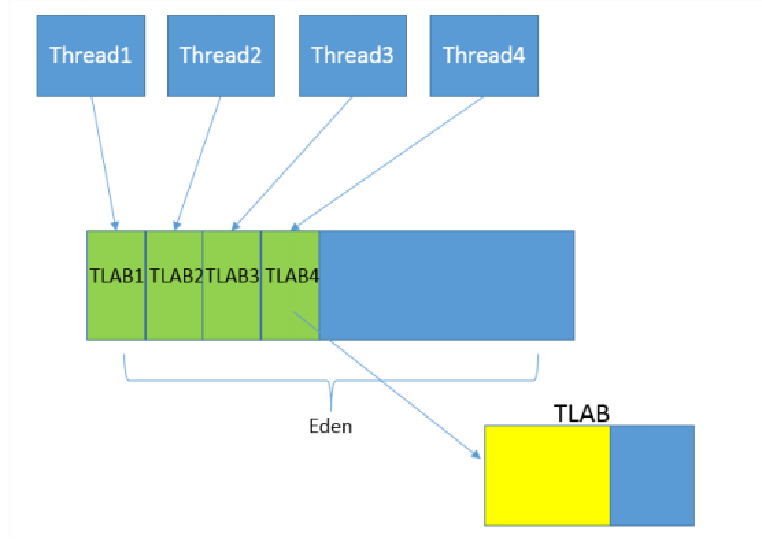
\includegraphics[width=\linewidth]{figures/TLAB}
  \caption{Thread Local Allocation Buffer}
\end{figure}

\section{Evaluation}
We evaluate our desgin by allocating memory pages, and we use representative big data processing frameworks Flink to verify the feasibility of our implementation.
The result shows that, compared with orginal G1 GC, our implementation could achieve shorter execution time and GC pause time, less object movement and remember set
footprint without negative effect on other functions.

\subsection{Evaluation Setup}

\subsection{TLAB Size}

\subsection{GC Pause Time}


%%
%% The next two lines define the bibliography style to be used, and
%% the bibliography file.
\bibliographystyle{ACM-Reference-Format}
\bibliography{mybib}

\end{document}
\endinput